\subsection{Profile Module}
\label{sec:mobile-profile}

\textbf{Purpose:}
Provides a centralized interface for managing user account information and application preferences. The Profile module enables authenticated users to view their personal information, customize application settings, switch between light and dark themes, and securely terminate their session.

\vspace{0.2cm}
\noindent\textbf{Main Features}

\begin{itemize}
    \item View User Information
    \item Account Management
    \item Theme Switching
    \item Secure Logout
\end{itemize}

%%%%%%%%%%%%%%%%%%%%%%%%%%%%%%%%%%%%%%%%%%%%%%%%%%%%%%%%%%%%

\subsubsection{Profile Screen}

\textbf{Purpose:}
Displays the authenticated user's profile information together with the available account management options.

\begin{figure}[H]
    \centering
    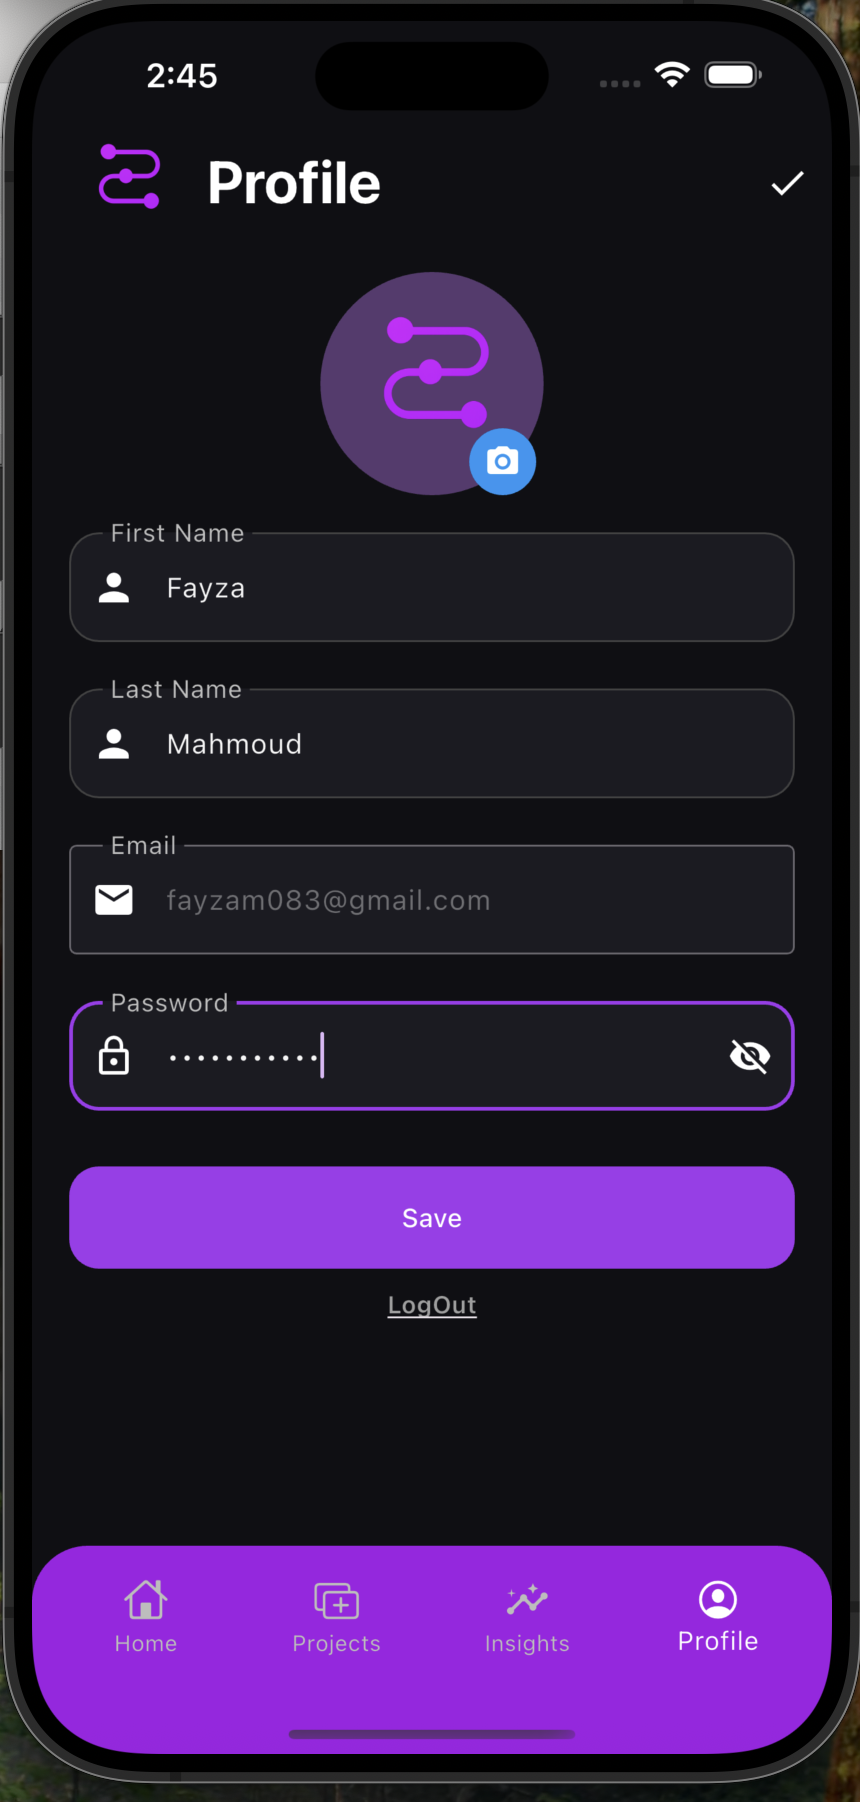
\includegraphics[width=0.42\textwidth]{images/mobile-app/admin-dashboard/profile-page-D.png}
    \caption{Profile Screen}
    \label{fig:mobile-profile}
\end{figure}

\vspace{0.2cm}
\noindent\textbf{Main Components}

\begin{itemize}
    \item User Avatar
    \item User Name
    \item Email Address
    \item Account Settings
    \item Theme Switch
    \item Logout Button
\end{itemize}

\vspace{0.2cm}
\noindent\textbf{Behavior \& Logical Flows}

\begin{itemize}
    \item Retrieves the authenticated user's profile information through authenticated REST API requests.
    \item Displays the user's personal information after successful data retrieval.
    \item Allows users to access account-related settings from a single interface.
    \item Updates the displayed information whenever profile data changes.
    \item Displays loading indicators while profile information is being fetched.
\end{itemize}

%%%%%%%%%%%%%%%%%%%%%%%%%%%%%%%%%%%%%%%%%%%%%%%%%%%%%%%%%%%%

\subsubsection{Theme Switching}

\textbf{Purpose:}
Allows users to personalize the application's appearance by switching between Light Mode and Dark Mode.

\vspace{0.2cm}
\noindent\textbf{Behavior \& Logical Flows}

\begin{itemize}
    \item Allows users to switch between light and dark themes.
    \item Stores the selected theme locally using SharedPreferences.
    \item Applies the selected theme immediately without restarting the application.
    \item Restores the previously selected theme automatically when the application is launched again.
\end{itemize}

%%%%%%%%%%%%%%%%%%%%%%%%%%%%%%%%%%%%%%%%%%%%%%%%%%%%%%%%%%%%

\subsubsection{Logout}

\textbf{Purpose:}
Provides a secure mechanism for terminating the current user session.

\vspace{0.2cm}
\noindent\textbf{Behavior \& Logical Flows}

\begin{itemize}
    \item Displays a confirmation dialog before logging out.
    \item Removes the stored JWT authentication token from local storage.
    \item Clears locally cached user information.
    \item Redirects users to the Login screen after successful logout.
    \item Prevents unauthorized access to protected application pages.
\end{itemize}

%%%%%%%%%%%%%%%%%%%%%%%%%%%%%%%%%%%%%%%%%%%%%%%%%%%%%%%%%%%%

\subsubsection{Profile State Management}

\textbf{Purpose:}
Maintains synchronization between the mobile application and backend services while ensuring a responsive user experience.

\vspace{0.2cm}
\noindent\textbf{Behavior \& Logical Flows}

\begin{itemize}
    \item Loads user profile information during page initialization.
    \item Handles loading, success, and error states while communicating with the backend.
    \item Updates the interface automatically after receiving backend responses.
    \item Maintains the user's authenticated session throughout application usage.
    \item Refreshes profile information whenever changes are detected.
\end{itemize}